% !TeX spellcheck = de_DE
% !TeX program = lualatex
\documentclass{alex_hü}
\usepackage{tikz-feynman}

\name{Alexander Helbok}
\course{PS Physik}
\hwnumber{12}


\begin{document}
\renewcommand{\labelenumi}{\alph{enumi})}
\renewcommand{\labelenumii}{(\arabic{enumii})}


\begin{mybox}{Feynman-Diagramme}
	\begin{enumerate}
		\item \ch{e- + e- -> e- + e-}\\[2ex]
		\feynmandiagram [horizontal=a to b] {
			i1 [particle=\(e^{-}\)] -- [fermion] a,
			i2 [particle=\(e^{-}\)] -- [fermion] a,
			a -- [photon, edge label=\(\gamma\)] b,
			b -- [fermion] f2 [particle=\(e^{-}\)],
			b -- [fermion] f1 [particle=\(e^{-}\)],
		};
	\tcbline
		\item \ch{\( \gamma \) + e- -> \( \gamma \) + e-}\\[2ex]
		\feynmandiagram [horizontal=a to b] {
			i1 [particle=\(e^{-}\)] -- [fermion] a,
			i2 [particle=\(\gamma\)] -- [photon] a,
			a -- [] b,
			b -- [photon] f2 [particle=\(\gamma\)],
			b -- [fermion] f1 [particle=\(e^{-}\)],
		};
	\tcbline
		\item \ch{e- + e+ -> \( \gamma \) + \( \gamma \)}\\[2ex]
		\feynmandiagram [horizontal=a to b] {
			i1 [particle=\(e^{-}\)] -- [fermion] a -- [fermion] i2 [particle=\(e^{+}\)],
			a -- [] b,
			b -- [photon] f2 [particle=\(\gamma\)],
			b -- [photon] f1 [particle=\(\gamma\)],
		};
	\tcbline
		\item \ch{p + e- -> n + \nu_e}\\[2ex]
		\feynmandiagram [horizontal=a to b] {
			i1 [particle=\(p\)] -- [fermion] a,
			i2 [particle=\(e^{-}\)] -- [fermion] a,
			a -- [boson, edge label=\(W^{+}\)] b,
			b -- [fermion] f2 [particle=\(n\)],
			b -- [fermion] f1 [particle=\(\nu_e\)],
		};
	\tcbline
%	\tcbbrea
		\item \ch{e- + e- -> W+ + W-}\\[2ex]
		\feynmandiagram [horizontal=a to b] {
			i1 [particle=\(e^{-}\)] -- [fermion] a -- [fermion] i2 [particle=\(e^{+}\)],
			a -- [] b,
			b -- [boson] f2 [particle=\(W^{+}\)],
			b -- [boson] f1 [particle=\(W^{-}\)],
		};
	\end{enumerate}
\end{mybox}

\begin{mybox}{W-Zerfall und Farbladung}
	\centering \(  \)
	\tcblower
	\begin{enumerate}
		\item \(  \)
%		\begin{flalign*}
	%			
%		\end{flalign*}
	\tcbline
		\item \(  \)
%		\begin{flalign*}
	%		
%		\end{flalign*}
	\end{enumerate}
\end{mybox}

\begin{mybox}{Teilchenidentifikation}
	\begin{enumerate}
		\item \(  \)
		\begin{tabular}{c@{\extracolsep{0.5cm}} c c c c c || c c }
			& \( Q \) & \( S \) & \( C \) & \( \tilde{B} \) & \( Y \) & \( B \) & Quarks \\
			\midrule
			(1) & \( 0 \) & \( 0 \) & \( 0 \) & \( 0 \) & \( 1 \) & \( 1 \) & \( udd \) \\
			(2) & \( 1 \) & \( 1 \) & \( 1 \) & \( 0 \) & \( 2 \) & \( 0 \) & \( \bar{s}c \) \\
			(3) & \( 0 \) & \( -1 \) & \( 0 \) & \( 0 \) & \( -1 \) & \( 0 \) & \( s\bar{d} \) \\
			(4) & \( -1 \) & \( -1 \) & \( 0 \) & \( 0 \) & \( 0 \) & \( 1 \) & \( sdd \) \\
			(5) & \( 0 \) & \( -1 \) & \( 0 \) & \( 0 \) & \( 0 \) & \( 1 \) & \( sud \) \\
			(6) & \( -1 \) & \( 1 \) & \( -1 \) & \( 0 \) & \( -1 \) & \( -1 \) & \( \bar{s}\bar{c}\bar{u} \) \\
		\end{tabular}
	\tcbline
		\item \(  \)
		\begin{enumerate}
			\item \( N(1520) \)
			\item \( D_s^{*+}(2112) \)
			\item \(  \)
			\item \( \Sigma(1385) \)
			\item \( \Lambda(1600) \)
			\item \( \bar{\varXi}_c^+(2468) \)
		\end{enumerate}
	\tcbline
		\item \( I_{N} = \tfrac{1}{2};\quad I_{\Delta} = \tfrac{3}{2} \) \\[2ex]
		\begin{tikzpicture}
			\definecolor{crimson}{HTML}{DC143C};
			\node[anchor=south west,inner sep=0] at (0,0) {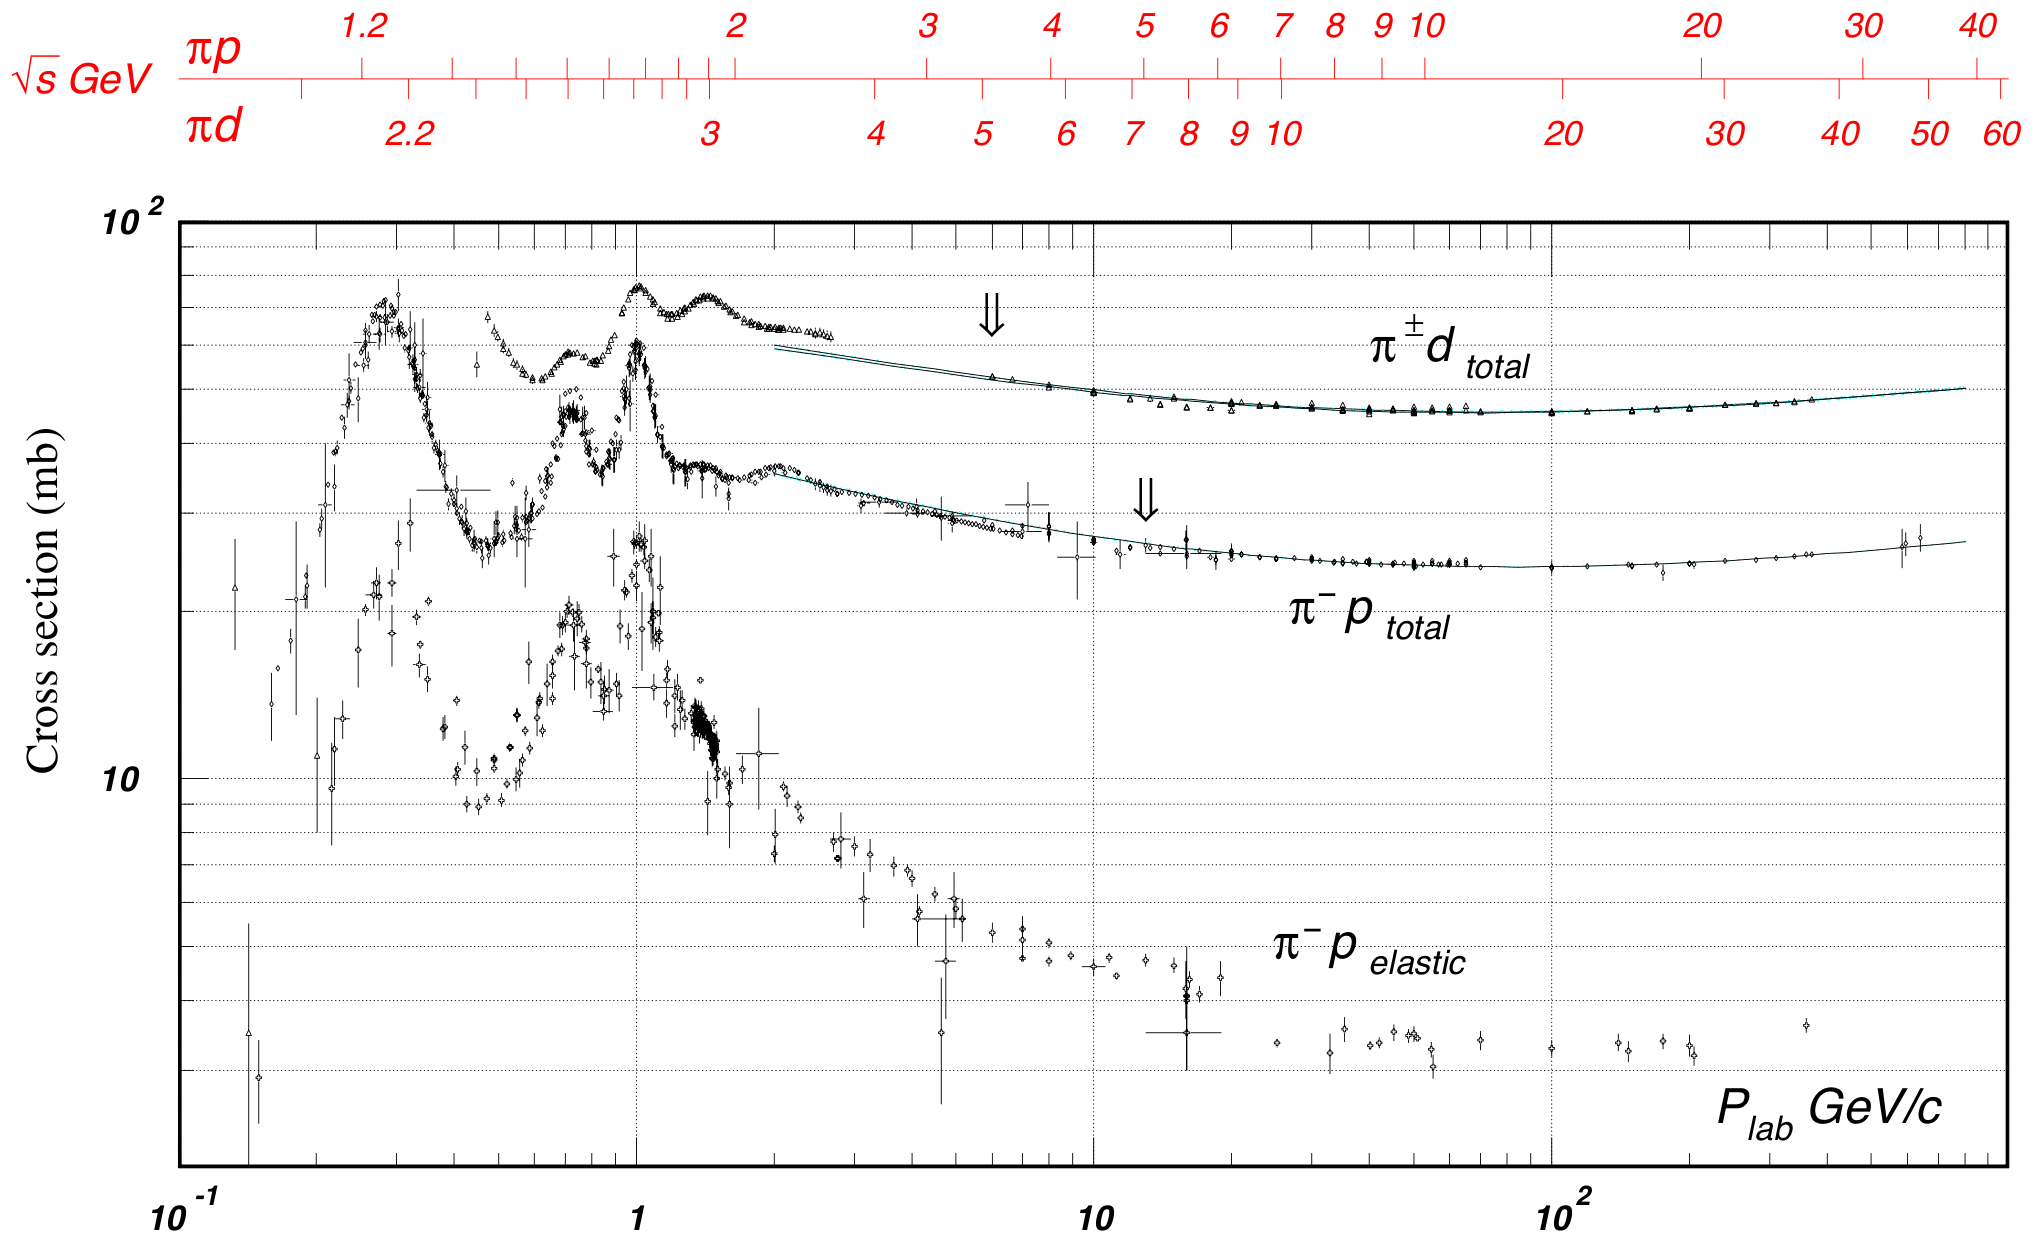
\includegraphics[width=0.85\textwidth]{resonance}};
			\draw[thick, -latex, crimson] (2, 4.8) -- (2.5, 5.8) node [pos=0, below] {\footnotesize \( \Delta(1232) \)};
			\draw[thick, -latex, crimson] (5, 4) -- (3.8, 5.2) node [pos=0, below right] {\footnotesize \( N(1520) \)};
		\end{tikzpicture}
		
		Es treten Resonanzen mit \( I = \tfrac{1}{2} \) und \( I = \tfrac{3}{2} \) auf, da die Kombination von \( I_\pi = 1 \) und \( I_p = \tfrac{1}{2} \) gemäß \( I_{\text{ges}} \in \{ \abs{I_\pi - I_p}, \abs{I_\pi + I_p} \} \) sowohl auf \( \tfrac{1}{2} \) als auch auf \( \tfrac{3}{2} \) führt. 
	\end{enumerate}
\end{mybox}


\end{document}